\documentclass{article}
\usepackage[utf8]{inputenc}
\usepackage{graphicx}
\usepackage{titling}
\usepackage{pgfgantt}
\usepackage{pdflscape}
\usepackage{hyperref}
\usepackage{animate}
\usepackage{movie15}

\renewcommand{\refname}{Kaynakça}
\pretitle{
  \begin{center}
  \LARGE\bfseries
  
\includegraphics[width=0.1\textwidth]{logo.png} 
  \vskip 1em
}
\title{Yapay Zeka ile Görüntü Gürültüsü Azaltma Projesi}
\author{İlyas Cemal Erginli}
\date{Mart 2024}

\begin{document}
\begin{titlepage}
    \maketitle
    \begin{center}
        \includegraphics[width=0.8\textwidth]{imageAı.jpg}
    \end{center}
    \thispagestyle{empty}
    \vfill
    \rule{\textwidth}{0.5pt}
    \renewcommand{\abstractname}{Özet}
    \begin{abstract}
    \noindent Bu projenin amacı, gürültülü görüntülerdeki istenmeyen gürültüyü azaltarak veya ortadan kaldırarak daha net ve kaliteli görüntüler elde etmektir. Bu proje, çeşitli alanlarda (örneğin, tıbbi görüntüleme, fotoğrafçılık, video işleme) kullanılabilecek, gürültülü görüntülerin kullanışlılığını artırmayı hedefler. Yapay zeka modelleri, gürültülü görüntülerdeki desenleri ve yapıları tanıyarak gürültüyü azaltmak için öğrenilmiş bilgiyi kullanır. Bu proje, daha iyi görsel kalite ve daha doğru analiz sonuçları elde etmek için gürültülü görüntülerin iyileştirilmesine odaklanır.
    \end{abstract}
    \rule{\textwidth}{0.5pt}
    \vfill
\end{titlepage}

\newpage
\section{Giriş}
\rule{\textwidth}{0.5pt}\\[10pt]
Günümüzde, dijital görüntüleme teknolojileri hızla gelişmekte ve yaygın bir şekilde kullanılmaktadır. Ancak, bu teknolojilerin kullanımında sıkça karşılaşılan bir sorun da görüntülerin gürültülü olmasıdır. Gürültü, birçok faktörden kaynaklanabilir ve görüntülerin kalitesini düşürerek bilgi kaybına neden olabilir. Bu nedenle, görüntü gürültüsünün azaltılması, görüntüleme teknolojilerinin etkinliğini artırmak ve veri analizi süreçlerini iyileştirmek için önemli bir gerekliliktir. \\[10pt]

 \noindent Bu proje, yapay zeka tekniklerini kullanarak görüntü gürültüsünün azaltılmasını hedeflemektedir. Yapay zeka, özellikle derin öğrenme teknikleri, karmaşık veri yapılarını işleyebilme yetenekleriyle gürültü azaltma işlemlerinde etkili bir şekilde kullanılmaktadır. Bu proje kapsamında, gelişmiş yapay zeka algoritmaları ve derin öğrenme modelleri, gürültülü görüntülerin temizlenmesi için kullanılacak ve daha net ve kaliteli görüntüler elde edilmesi sağlanacaktır.\\[10pt]

\section{Literatür Çalışması}
\rule{\textwidth}{0.5pt}

 \noindent Bu makalede\cite{zhang2018ffdnet}, Hızlı ve etkili bir görüntü gürültü giderme yöntemi olan FFDNet, ayırt edici öğrenme yöntemlerinden farklı olarak geniş bir gürültü seviyesi aralığını tek bir ağla ele alabilir. Esnek bir yapıya sahip olan FFDNet, giriş olarak ayarlanabilir bir gürültü seviye haritası kullanarak mekansal olarak değişken gürültüyü de çıkarabilir. Ayrıca, örnekleme yapılmış alt görüntüler üzerinde çalışarak hızlı çıkarım hızı sağlar ve BM3D'e kıyasla daha hızlı sonuçlar elde eder. Yapılan deneyler, FFDNet'in etkili ve verimli olduğunu göstermiştir, bu da pratik gürültü giderme uygulamaları için cazip bir seçenek haline getirir.\\[10pt]

 \noindent Bu makalede\cite{yu2019deep}, Düşük seviye görüş araştırmalarında yaygın olarak incelenen özellik haritalarının indirme ve yükleme ölçeklendirme kullanılarak ağlar, verimli GPU bellek kullanımı ve geniş duyarlı alanları sağlama kapasiteleri nedeniyle incelenmiştir. Bu bağlamda, görüntü gürültü giderme için derin tekrarlayan indirme-yükleme evrişimli sinir ağı (DIDN) önerilmektedir. Bu ağ, özellik haritalarının çözünürlüğünü tekrar tekrar azaltıp artırır. Ağın temel yapısı, özgün olarak anlamsal segmentasyon için geliştirilen U-Net'ten esinlenmiştir. İndirme ve yükleme katmanları, görüntü gürültü giderme görevi için uyarlanmıştır. Geleneksel gürültü giderme ağları, tek seviyeli gürültüyle çalışması için eğitilmiştir veya alternatif olarak, tek bir modelle çoklu seviyeli gürültüyü ele almak için gürültü bilgisini giriş olarak kullanır. Bununla birlikte, ağımızın etkili bellek kullanımı, tek bir modelle gürültünün geniş bir aralığını işlemesini sağlar ve bu da gürültü bilgisi girişlerine ihtiyaç duymadan çoklu seviyeli gürültüyü ele almasını sağlar. Sonuç olarak, DIDN, referans veri kümesinde en son teknoloji performansını sergiler ve aynı zamanda NTIRE 2019 gerçek görüntü gürültü giderme yarışmasında üstünlüğünü gösterir.\\[10pt]




\newline
\noindent
\section{Yöntemler}
\rule{\textwidth}{0.5pt}
Bu projede, Convolutional Neural Network (CNN) gibi derin öğrenme yöntemleri yanı sıra, temiz veri oluşturma için kullanılan autoencoder gibi unsupervised öğrenme teknikleri de kullanılacaktır. Autoencoder'lar, gürültülü görüntüyü giriş olarak alıp, gizli katmanlarda temiz görüntüyü oluşturarak gürültü azaltma sürecini gerçekleştirirler. Ayrıca, gürültülü görüntülerdeki istenmeyen özelliklerin tanımlanması için denetimli öğrenme yöntemleri de uygulanabilir. Bu yöntemlerde, gürültülü ve temiz görüntülerin eşleştirildiği bir eğitim veri seti kullanılarak, gürültülü görüntülerden temiz görüntülerin tahmini için öğrenme gerçekleştirilir.\\[10pt]

 \noindent Bu farklı yöntemlerin kombinasyonu, gürültü azaltma sürecindeki etkinliği artırabilir ve çeşitli gürültü tipleriyle başa çıkabilme kabiliyetini sağlayabilir. Autoencoder'lar, gürültülü verilerden temiz verilerin oluşturulmasında kullanılarak, CNN'lerin daha iyi performans göstermesine yardımcı olabilir. Denetimli öğrenme yöntemleri ise belirli gürültü tiplerine özgü özelliklerin tanımlanması ve gürültü azaltma işleminin hassaslaştırılması için önemli bir rol oynar. Bu yöntemlerin bir araya getirilmesi, daha güçlü ve esnek bir gürültü azaltma çözümü elde etmek için önemlidir.\\[10pt]

 \section{Veri Odaklı Sistem Tasarımı}
\rule{\textwidth}{0.5pt}

 \noindent Veri odaklı bir sistem tasarımı, yapay zeka algoritmalarının kullanıldığı herhangi bir projede temel bir kavramdır. Görüntülerdeki gürültüyü azaltma projesinde de bu kavram önemlidir. Bu tasarım, veriye dayalıdır çünkü gürültüyü azaltmak için modelin öğrenmesi gereken temel bilgileri içerir.\\[10pt]

 \noindent İlk olarak, projenin başlangıcında, geniş bir veri kümesi toplanır. Bu veri seti, gürültülü ve gürültüsüz görüntüler içerir. Gürültü seviyeleri farklı koşullarda değişebileceğinden, çeşitli ortamlarda ve çeşitli koşullarda çekilmiş görüntüler içermesi önemlidir. Bu veri, modelin genelleme yeteneğini artırır ve gerçek dünya uygulamalarında daha etkili sonuçlar elde etmesini sağlar.\\[10pt]

\noindent Daha sonra, toplanan veri kümesi önceden işlenir ve etiketlenir. Gürültülü ve gürültüsüz görüntüler birbirinden ayrılır ve modelin öğrenme sürecinde doğru geribildirim sağlamak için uygun etiketlerle eşleştirilir. Bu adım, modelin doğru bir şekilde gürültüyü tanımasını ve gidermesini sağlar.\\[10pt]

\noindent Veri odaklı sistem tasarımının bir sonraki aşaması, modelin eğitimini içerir. Bu aşamada, derin öğrenme gibi yapay zeka teknikleri kullanılarak, model gürültülü görüntülerden gürültüsüz versiyonlarını oluşturmayı öğrenir. Eğitim süreci boyunca, model toplanan veri kümesi üzerinde iteratif olarak eğitilir ve geliştirilir.\\[10pt]

 \noindent Son olarak, eğitilen model test edilir ve kullanıma hazır hale getirilir. Test aşamasında, modelin performansı belirlenir ve gerçek dünya verileri üzerinde doğru sonuçlar üretip üretmediği değerlendirilir. Modelin başarılı olduğu gözlemlendiğinde, kullanıcıların kullanımına sunulabilir.\\[10pt]

 \noindent Bu veri odaklı sistem tasarımı yaklaşımı, yapay zeka ile görüntülerdeki gürültüyü azaltma gibi karmaşık problemlerin etkili bir şekilde çözülmesine olanak sağlar. Veriye dayalı modelleme ve eğitim süreci, modelin gerçek dünya verilerinde genelleme yapmasını sağlar ve daha iyi sonuçlar elde edilmesine yardımcı olur.\\[10pt]


\section{Proje İçerik   Aşamaları}
\rule{\textwidth}{0.5pt}

\subsection{Problem Belirleme ve Tanımı}
Görüntü gürültüsünü azaltma problemiyle ilgili belirli bir hedef belirlenir. Bu hedef genellikle, gürültülü bir görüntüden mümkün olduğunca temiz bir görüntü elde etmeyi içerir.
Gürültü türleri belirlenir. Örneğin, görüntülerdeki yaygın gürültü türleri arasında Gaussian gürültü, salt-and-pepper gürültü ve speckle gürültü bulunur.

\subsection{Literatür İncelemesi}
 Benzer projelerde kullanılan yöntemler, algoritmalar ve teknikler incelenir.
Mevcut literatürden elde edilen bilgiler, projenin temelini oluşturur ve bu bilgiler doğrultusunda ilerlenir.

\subsection{Veri Toplama ve Hazırlığı}
Bu aşamada, gürültülü ve temiz görüntü çiftlerinden oluşan bir veri seti toplanır. Bu veri seti, modelin eğitimi ve değerlendirmesi için kullanılacaktır.
Veri ön işleme adımları gerçekleştirilir. Bu, görüntülerin boyutlarını standartlaştırma, renk kanallarını düzenleme, gürültü ekleme ve benzeri işlemleri içerebilir.

\subsection{Algoritma Seçimi ve Model Geliştirme:}
Gürültü azaltma için kullanılacak yapay zeka algoritmaları gözden geçirilir. Bu genellikle evrişimli sinir ağları (CNN'ler), otomatik kodlayıcılar (autoencoders) veya derin öğrenme tabanlı diğer yöntemleri içerir.
En uygun algoritma veya algoritmalar seçilir ve bir model mimarisi tasarlanır. Bu, ağın katmanlarının ve hiperparametrelerinin belirlenmesini içerir.



\subsection{Model Eğitimi}
Tasarlanan model, gürültülü ve temiz görüntü çiftleri üzerinde eğitilir.
Eğitim sırasında, model gürültülü görüntüleri girdi olarak alır ve temiz görüntüleri hedef olarak kullanır. Model, bu girdi-çıktı ilişkisini öğrenmeye çalışır.
Modelin performansını ölçmek için eğitim ve doğrulama veri setleri kullanılır. 

\subsection{Model Değerlendirmesi}
Eğitilmiş model, ayrı bir test veri seti üzerinde değerlendirilir. Bu, modelin gerçek dünya verileri üzerinde nasıl performans gösterdiğini belirlemeye yardımcı olur.
Modelin performansı, belirlenen metrikler (PSNR, SSIM, MSE gibi) kullanılarak ölçülür.

\subsection{Sürekli İyileştirme ve Bakım}
Modelin performansı düzenli olarak izlenir ve değerlendirilir. Gerekirse, model güncellemeleri yapılır ve yeniden eğitilir.
Geri bildirimlerve değişen gereksinimler doğrultusunda model ve sistem iyileştirmeleri yapılır. Bu, yeni veri toplama, modelin yeniden eğitimi veya algoritma değişikliklerini içerebilir.

 \begin{landscape}
\thispagestyle{empty} % Sayfa numarasını kaldırmak için
    \begin{figure}
     \centering
  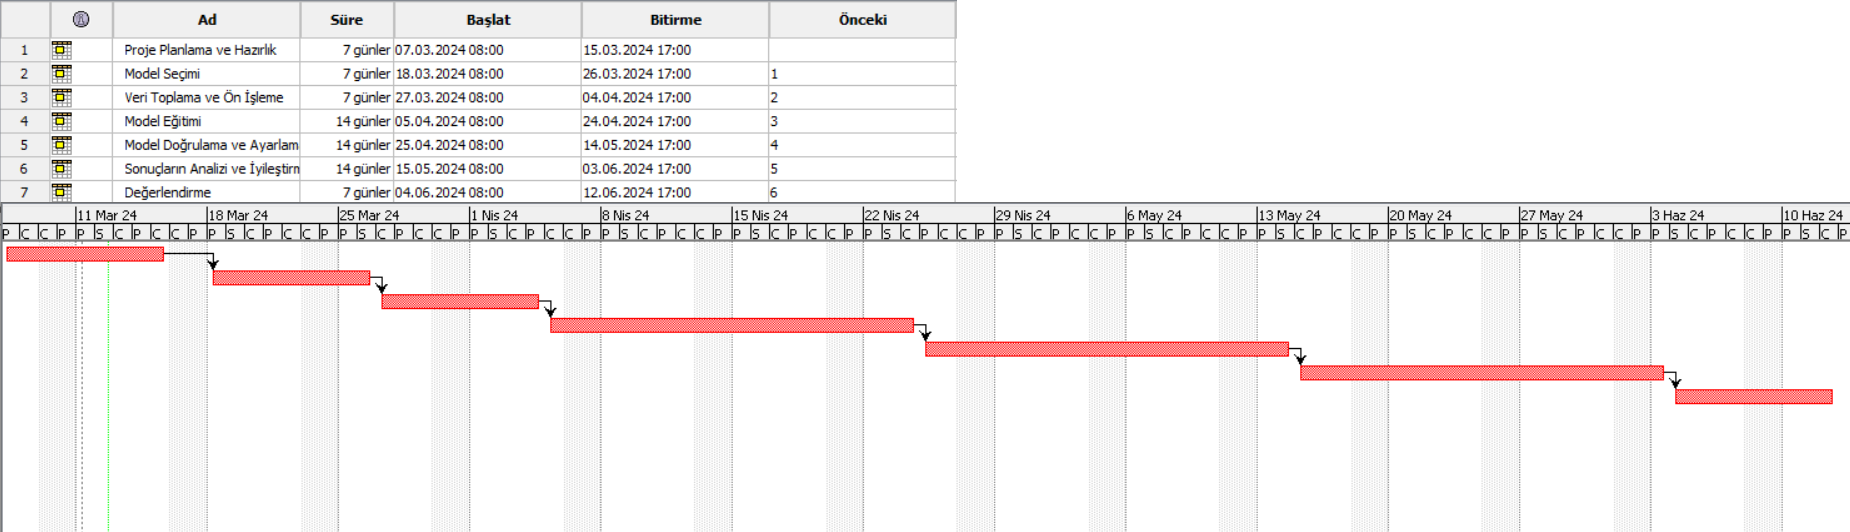
\includegraphics[angle=360,width=1.6\textwidth]{gantt_chart.png}\centering % Resim dosyasının adını ve uzantısını belirtin
  \caption{Gantt Chart}
  \label{fig:resim_etiketi}
\end{figure}

    % Yana çevirmek istediğiniz içerik buraya gelir
\end{landscape}

\bibliographystyle{ieeetr}
\bibliography{alıntı}

\end{document}



